\documentclass[12pt]{report}
\usepackage[utf8]{inputenc}
\usepackage{graphicx}
\usepackage[tmargin=2cm, lmargin=4cm, rmargin=2.5cm, bmargin=4cm, paperwidth=8.267in, paperheight=11.692in]{geometry}
\usepackage{amsfonts}
\usepackage{array}
\usepackage{indentfirst}
\graphicspath{ {images/} }
\usepackage{lipsum}
\usepackage{verbatim}
\usepackage{titlepic}
\usepackage{amsmath}
%\usepackage{titlesec}

\begin{document}

\title{Light Field Research \vspace{2.5cm}}	%\includegraphics[scale=0.2]{university_edinburgh.jpg}
\author{
\Large Carson Vogt \vspace{1cm} \\ 
}

\date{
	\centering
	PhD \endgraf\medskip
	Heriot-Watt University \endgraf\medskip
	20 January 2017
}

\maketitle

\listoffigures

\tableofcontents

\chapter{Introduction}
Light field rendering is a fascinating image-based rendering (IBR) technique whose properties have only begun to be explored. With the seminal paper on the topic relatively recently published in 1996 by Levoy and Hanrahan\cite{Levoy96}, research and applications have been rather limited. Early research was focused largely on improving graphics as IBR provides a very immersive and potentially fluid experience for the user, while theoretically relying on very little information of the scene, such as geometry. Of course, as will be discussed, there are times when having extra information like scene geometry can be useful in rendering \cite{Gortler96}. Partly due to the original purpose behind light fields, current research trends have largely been directed towards virtual reality (VR) applications in the entertainment industry \cite{Anderson16, Davis12, Kalantari16}. Apart from attempts at applying light fields to microscopy and depth estimation, few researchers have successfully attempted to apply the light field methodology to other areas \cite{Levoy06b}. There are a number of reasons for the limited research directions and abundance which will be covered here as well as the positive aspects and advantages of light field IBR.

Light fields are a rising method for rendering scenes. With the increasing popularity of VR, light field technology has the potential to revolutionize the way in which viewers interact with subjects of interest.
\begin{figure}[!ht]
	\centering
	\includegraphics[scale=0.75]{levoy_lf.jpg}
	\caption{ \cite{Levoy96}.}
	\label{fig:levoy_lf}
\end{figure}
McMillan and Bishop describe IBR as the method of creating a "continuous representation" of a scene or subject being discretely sampled \cite{McMillan95}. The sampling that makes up light field IBR is derived from the plenoptic function, a seven-dimensional function that describes the sum of light rays at any point in space \cite{Adelson91}. However, the plenoptic function itself is rarely if ever used in practical applications or research as measuring the full plenoptic function would be impossible. The plenoptic function effectively stopped being used in research in its 7D form with \cite{Adelson91}, but from it the light field was created which allows for descrete parts of the plenoptic function to be measured.

The light field itself was presented by Levoy in 1996 and is a 4D function that is oftened viewed flattened as a 2D array of 2D images. An excellent example of this can be seen in figure \ref{fig:levoy_lf}, and was collected by Levoy and Hanrahan in their early research. After collecting these images, the light field is actually utilized by querying a database of light rays corresponding to the viewpoint of the observer. This requires the camera location to be known very precisely such that when the rays are actually collected and stored, the correct rays can then be utilized when creating the new view. While this is how the methodology is presented in the literature, the story for practical applications is different, and relies instead on a number of assumptions about the light field being collected and blending the resulting images, which will be covered later in the report.

Light fields have a number of intriguing qualities, some of which have yet to be fully exploited. As mentioned before, the most popular quality is the immersive nature of the light field. Taking real images naturally makes it more realistic so long as images are smoothly rendered from the database. another interesting quality comes about due to the large number of images acquired. Occluders within a scene can effectively be erased from the scene, as shown in figure \ref{fig:seethrough_occluder}. While no individual image captured can recreate a complete view of the background, the pieces of the background captured can be combined to recreate it, sometimes entirely removing the occluder from the scene \cite{Vaish06}.
\begin{figure}[!ht]
	\centering
	\begin{minipage}{0.45\textwidth}
		\centering
		\includegraphics[scale=0.55]{seethrough_occluder.png}
		\caption{}
		\label{fig:seethrough_occluder}
	\end{minipage}\hfill
	\begin{minipage}{0.45\textwidth}
		\centering
		\includegraphics[scale=0.55]{seethrough_occluder2.png}
		\caption{}
		\label{fig:seethrough_occluder2}
	\end{minipage}
\end{figure}

There are a number of major limitations associated with light fields currently. To attain the very immersive qualities that makes them appealing, a large number of images must be acquired. If image density is too low, several rendering artifacts can appear, such as hair, pixelation, etc cite{Camahort09}. Papers have been published to decrease the number of required images and will be covered in more detail in the \emph{Literature Review} chapter of the report. Because of the large number of images required, the method for data collection is often bulky or slow \cite{lfArchive}. The light field is further limited by the collectors chosen parameterization, and generally limits the viewer to a planar or spherically based view of the scene \cite{Levoy06a}. 

If one goes back to the original paper regarding the plenoptic function, a critical element is present in it and missing from the current parameterizations: time. Up until recently, light fields have been collected only for static scenes, but advances in light field cameras and processing power have seen small advancements in dynamic light fields \cite{Anderson16, lytro}. Regardless, this still leaves the user with the problem of mobility, where apparatus are fixed and generally must adhere to the strict parameterization around which they were designed. And still, the applications have only been for VR applications.

The project goal is two-fold: one part being to utilize existing research in novel ways to collect and allow for the visualization of dynamic light fields. The second part is to explore novel applications, such as visualizations for the medical field, sports, and other scientific areas such as botany that could benefit from a method of viewing subjects from any point in space \emph{and} time.

\chapter{Literature Review}
The light field is, at its base, a derivation of the plenoptic function (the root \emph{plenus} meaning complete). The plenoptic function, the concept for which was set forward by Adelson and Bergen in 1991, is a method of mathematically describing the elements of vision. The paper takes on the task of defining what can be seen across 3D space, where every point (or "pencil" of rays) contains the information for all of the rays passing through it. This is illustrated well in figure \ref{fig:plenoptic_visual}. 
\begin{figure}[!ht]
	\centering
	\includegraphics[scale=0.75]{plenoptic_image.png}
	\caption{The plenoptic function sampled at two points, showing all pencils of light rays which pass through those points \cite{Adelson91}.}
	\label{fig:plenoptic_visual}
\end{figure}
The concept of all light passing through a point is rooted in the early observations of Leonardo da Vinci, who observes the effect of a hole in a wall, which reveals an image of the scene in front of the wall, upside down on the back wall \cite{Adelson91}. This is the concept behind the pinhole camera, which is a key assumption applied to cameras in much of the work done with light fields. This allows for the use of a ray tracing technique regarding the incoming light rays to a camera. These rays can then be individually stored and queried at a future date for the synthesis of new or old views. The next section discusses the derivation of the 4D light field from the 7D plenoptic function.  

\section{Early Research and Derivation from Plenoptic Function}
Having a basic idea of what constitutes light in space, Adelson and Bergen set forth to mathematically represent this plenoptic function.
The function itself is given as 
\begin{equation}
P=P(\theta,\phi,\lambda,t,V_x, V_y,V_z)
\end{equation}
where $\theta$ and $\phi$ are the viewing angles from a point in space, $\lambda$ is the wavelength of the incoming ray, $t$ is the time parameter at which the ray is observed, and $V_x,V_y,V_z$ define the location in three dimensional space at which the incoming rays are measured \cite{Adelson91}. This defines the incoming rays at every point in 3D space for all time. This would then theoretically allow for the reconstruction of any view, in any space for which the plenoptic function was completely known or measured. However, measuring the plenoptic function comes with its own set of difficulties.

The 7D plenoptic function is a bit impractical to work with, and researchers sought, and continue to seek, to reduce the dimensionality of the function in a number of ways. In \cite{McMillan95} and \cite{Huang14}, the 7D plenoptic function is reduced to five dimensions,
\begin{equation}
p=P(\theta,\phi,V_x,V_y,V_z)
\end{equation}
where $t$ and $\lambda$ are omitted as the time of sampling is considered to be constant (therefore requiring the scene remain static) and the wavelength is constant so long as there are no occluders \cite{Levoy06a}. 

In Levoy and Hanrahan's seminal paper \emph{Light Field Rendering} \cite{Levoy96}, the authors note that in space free of occlusions, the function can be further reduced to a four dimensional function as the ray of light reaching the pixel will not be altered in free space. In this environment, the only requirement is to know the direction of a ray, which is a function of four points shown in the following equation:
\begin{equation}
r=L(u,v,s,t)
\end{equation}
where $r$ is the radiance of an individual ray passing through the planes. This parameterization requires a ray to pass through two known planes, defined as the $s,t$ and $u,v$ planes. This is  still a standard parameterization, used in \cite{Isaksen01}, \cite{Vaish06}, and \cite{Oberlin16}, among others. In one case, a three dimensional parameterization is used as acquisition is completed by using a 1D row of cameras, though obviously this is considerably more limiting than the previous cases, and is considerably less frequently used \cite{Kim13}. Levoy and Hanrahan introduce the 4D parameterization as the "light field" \cite{Levoy96}.

While \cite{Levoy96} introduces the popular two plane parameterization, McMillan and Bishop define a cylindrical parametrization a year earlier. Having encountered difficulties storing a spherical parameterization on a computer, the authors note that with a cylinder, it can effectively be unrolled into a plane, thus making it easy to store and access \cite{McMillan95}. While it may have been easier, it is quickly passed by spherical parameterizations, which offers viewers the ability to also look up. In \emph{Light Fields and Computational Imaging}, Levoy outlines the available parameterizations as of 2006, shown in figure \ref{fig:parameterization_visual}.

With Isaksen et al.'s \emph{Dynamically Reparameterized Light Fields}, a reworking, of the original two plane parameterization was developed, though \cite{Camahort09} argue that it is a separate parameterization altogether. Rather than have two planes in free space, the planes are moved to the internals of the camera, between the lens and the image sensor, guaranteeing the one of the original assumptions, that the space between the subject and the camera be free of occlusions. As well, the authors introduce the concept of not only a mobile focal plane, such as that seen in figure \ref{fig:mobile_focus}, but a focal plane free to change shape and distance according to the user \cite{Isaksen01}. 

\begin{figure}[!ht]
	\centering
	\includegraphics[scale=0.75]{Light-field-parameterizations.png}
	\caption{This image depicts the most common parameterizations at the time ***cite was written. Of the three, the two plane parameterization on the far right persists as the most popular.}
	\label{fig:parameterization_visual}
\end{figure}

\section{Light Field Collection}
Light field collection has gone relatively unchanged since its inception. Most techniques are a fairly brute force method utilizing a large array of cameras in one form or another. Stanford's New Light Field Archive uses a wall of cameras or a single camera on a gantry, while companies such as Lytro have developed a spherical bank of cameras. While there are some interesting methods for the collection of light fields, there are still quite limited by their parameterizations and the density of the data they must collect. 

The primary method by which light fields are captured is a brute force method relying on a large array of cameras \cite{Ng06}**. An example of this can be seen in figure \ref{fig:camera_array}. This method of capture allows for the light field to be captured quickly and precisely since each camera can capture an image at the same time as every other camera, and the location of each camera is known. However, due to the structure's vast size, moving it to capture interesting scenes is highly impractical, relying on the user to provide huge amounts of power and computing power to an impractical location outside of a lab. While a number of groups have shown interesting use cases for the camera array (some of which will be covered in later sections) such as \cite{Ng06}*****, it is clearly not a practical method for capturing difficult scenes.

In an effort to decrease the size and complexity of the system, the team at Stanford created a computer controlled, gantry-based, light field collection system \cite{Koller04}. This allowed the them to avoid using a complex and relatively immobile capture system in favor of a light and cheap single camera system. Of course, the gantry system is only appropriate for scenes that are static long enough for the camera to move through its programmed range of motion. It also removes some of the functions made possible by the array, such as high speed video from multiplexed cameras \cite{Wilburn05}.

Utilizing the growing capabilities of image sensors, Ng shows in his thesis a way by which a light field can be captured by a single camera. Rather than producing a single image, a microlens array is inserted into the camera, after the lens and before the image sensor (see figure). This enables the user to create such effects as refocusing and some minimal movement around the image for a 3D effect after the image has been captured \cite{Ng06}. The light field camera still suffers from a lack of **spatial and angular resolution, leaving room for research to be done combining the light field camera and novel collection techniques.

Another unique data collection method was demonstrated in Davis \emph{et al's} paper, \emph{Unstructured Light Fields} from 2012 \cite{Davis12}. In it, Davis 
Unstructured light fields paper also shows a method for collection utilizing a single camera and a SLAM algorithm known as PTAM(cite PTAM paper). Of course, this research is now a bit aged and can be improved in a number of ways, potentially expanding it significantly with the addition of a more robust and wide-ranging(?) SLAM method such as ORB-SLAM2(cite)

Minimizing the amount required to collect(cite review and actual article)
Move on to the more recent papers of Sparse lightfields and learning 
based view synthesis

\cite{Ng06}
\cite{Davis12}
\cite{Oberlin16}


While light field rendering is the most immersive image-based rendering technique, one of the drawbacks of the light field is that the number of images required to create a high resolution and immersive scene can be prohibitively large \cite{Anderson16}. This leads to the natural question of the amount of sampling required for a complete or usable light field. There's surprisingly limited number of papers on the subject, which likely has to do with the methods for data collection, and thus it is one of the less-studied areas within the light field field.

\section{Image Interpolation}
As mentioned, one of the drawbacks of light fields is the amount of data required. Without any data interpolation, collection must be very dense, requiring the impractical apparatus mentioned previously. A number of researchers have sought out a solution to the high density issue associated with the hopes of making the acquisition process faster. These methods vary from geometric analysis of light field collection to employing deep learning techniques to interpolate between collected images.

In the paper \emph{Plenoptic Sampling}, Chai et al. set about to describe a minimum sampling rate such that the light field might be completed without any image interpolation. Their method suffers from a rather large flaw, which is that they require the minimum and maximum depths within a scene, and assume that the method for collection is a 2D camera array. Regardless, they manage to present a minimum sampling between cameras in the array given in terms of the resolution of the sampling cameras and renderer (which is assumed to be equal) $\Delta v$ and $\delta v$, and the highest frequency computed from the spectral support $B_v^s$ \cite{Chai00}. 
\begin{equation}
\Delta t_{max} = frac{1}{min \left(B_v^s, 1/(2 \Delta v), 1/2 \delta v)\right) }
\end{equation}

Several other publications make use of geometry when collecting data for a light field. In Gortler***s paper, \emph{The Lumigraph}, it is noted that fewer images are required if the collector has some knowledge of the geometry of the scene \cite{Gortler96}. This concept is also made use of in more recent papers, such as \cite{Kim13}. However, such methods are limiting, especially from the persective of collecting the light field. Ideally, collecting the data should be as hands off as possible. For the purpose of this project the geometric methods are noted, but will not likely be used right away. 

In terms of post processing methods involving image interpolation, there have been a number of relatively new papers which seek to both minimize the number of images taken at the time of collection as well as fluidly complete the light field. In \cite{Shi14}, by analyzing the sparsity in the continuous Fourier domain, show that if light fields are collected to optimize for this, the number of images required to create a light field may be drastically reduced.

In 2016, a paper was published that described a method for employing deep learning to the problem of both collection and then completing the light field. Kalantari et al. trained convolutional neural networks on new view synthesis within light field cameras. Their results suggest that their method, at least on the small scale of a light field camera, produces superior images compared with the previous state of the art. An interesting note by the authors is that, unlike previous methods, use of the CNN means that the new images also carry over the camera artifacts. So while the images themselves might not necessarily be better than previous methods, they do blend in with the real images that were collected by the camera\cite{Kalantari16}. Some very interesting future work would consist of applying this to large scale light fields that might have been collected by robots.

Rendering may be viewed as a reconstruction
of the light field forming an estimate of the
perceived image around the objects
(Kriging Paper)

\section{Application of Light Fields}
Graphics and virtual reality are the most obvious applications for light fields and have effectively spurred on the field since the middle of the 1990s.

\begin{figure}[!ht]
	\centering
	\begin{minipage}{0.45\textwidth}
		\centering
		\includegraphics[scale=0.9]{stanford_camera_array.png}
		\caption{The dense camera array used at Stanford to capture a number of light fields.}
		\label{fig:camera_array}
	\end{minipage}\hfill
	\begin{minipage}{0.45\textwidth}
		\centering
		\includegraphics[scale=0.5]{lego_gantry.jpg}
		\caption{Another collection method, the gantry effectively mimics the camera array so long as the scene is not altered between gantry locations.}
		\label{fig:lego_gantry}
	\end{minipage}
\end{figure}

Riding on the work of Ng and the light field camera, Levoy \emph{et al} struck again with a paper on light field microscopy.\cite{Levoy06b}

In \cite{Vaish06} Vaish \emph{et al} utilize a large camera array to Demonstrate a method by which occlusions can effectively be removed if the light field is sampled densely enough, comparing several different techniques.

Some research has been done in light field videography, but it has been largely untouched. Wilburn \emph{et al}, utilizing a dense camera array, create a method for creating a high framerate system. However, the large camera array comes with its own set of problems in the form of.. It is not until 2016 that Google in a paper by Anderson \emph{et al} demonstrated effective light field video, bringing the generally left out time dimension back into the parameterization \cite{Anderson16}. 

It was Davis \emph{et al} who attempted to bring light fields to a consumer level outside of the light field camera concept put forward by Ng. While the use cases are limited, they went as far as developing an app that allowed users to capture their own light field and extract subjects from it as 3D objects \cite{Davis12}. Using a spherical parameterization, Davis \emph{et al} construct a light field by guiding a user with a graphical user interface that instructs the user on where to hold the camera for data collection.

Working at about the same time as Davis \emph{et al}, Jachnik \emph{et al} create a very similar system. While there are differences in user interface, and algorithmic difference, the concept is quite similar. However, after capturing a light field, the authors attempt to create a crude environment map, and from that the locations of light sources. The results are unique in that for augmented reality applications, shadowing can be implemented on an object that has been placed into a scene, creating a greater sense of realism \cite{Jachnik13}.

\section{Future Collection Methods}
With a few exceptions, the direction of light field capture has largely been constant with researchers relying on the large camera array depicted in figure*** While there have been other methods, such as those of Ng, Davis \emph{et al}, and Jachnik \emph{et al}, they are either limited in their spatial and angular representations, or require significant human interaction to actually create the light field.

 \cite{Oberlin16} demonstrated the ability to caputure a light field with a seven degree of freedom robot arm on a Baxter robot. While there is no doubt that this is a definite move from traditional collection methods, there is a vast amount of research yet to be done in this area with wide ranging applications that could bring light fields to industries outside gaming or virtual reality as attempted in \cite{Levoy06b}.

The current trend for light field cameras seems to be going in the direction of multi-camera mobile aparatus, as shown in figure \ref{fig:lytro_immerge}
The use cases for these capture methods are limited
\begin{figure}[!ht]
	\centering
	\begin{minipage}{0.45\textwidth}
		\centering
		\includegraphics[scale=0.08]{lytro_immerge.jpg}
		\caption{the lytro immerge, designed to capture an entire scene at once, with an array of cameras built into the structure.}
		\label{fig:lytro_immerge}
	\end{minipage}\hfill
	\begin{minipage}{0.45\textwidth}
		\centering
		\includegraphics[scale=0.12]{jump_vr_video_cameras.jpg}
		\caption{On the right is the camera rig behind the Google Jump VR video system \cite{Anderson16}}
		\label{fig:jump_cameras}
	\end{minipage}
\end{figure}. 

As noted in the introduction, part of the goal of this project is to be able to collect light fields via cameras mounted on one or multiple multirotors, such as the one pictured in ***figure. The amount of research that has gone into multirotor navigation and use as a tool is substantial. A number of those papers were reviewed which could pertain to their use a light field collection devices, covering topics such as trajectory, localization, and data collection. 

In the first, the previously mentioned PTAM system is integrated into a new navigation system, allowing for fairly accurate localization of the multirotor \cite{Engel12}.

In another paper, the authors*** were interested in aircraft placement for optimum lighting effects in a scene... \cite{Srikanth14}

The final paper with In another, a system was developed to define the trajectory of a multirotor... \cite{Roberts16}

\section{Light Field Photography}
This section goes through, in greater detail, a paper of particular interest written by Ng et al entitled \emph{Light Field Photography with a Hand-held Plenoptic Camera} \cite{Ng05}. In it, the authors outline a method for collecting light fields with a single, modified camera. Using this particular camera allows the authors to avoid the bulky and difficult camera array mentioned previously, while retaining the speed the single traditional camera apparatus loses.

A light field (or plenoptic) camera is virtually the same as a standard camera, with a few very important differences. As with many technologies, image sensors have grown in capability. Sensors of tens of megapixels are not uncommon, and it is this effective over-abundance of sensing power that allows the light field camera to operate. Instead of light going directly to the image sensor to create one large image, light from the lens first encounters a microlens array, which then creates smaller images on the image sensor. Because of this rather major change to the hardware of the camera, software changes must also be made to render images that make use of the modified output from the image sensor. The light field camera can then be thought of as a miniaturized version of the camera array mentioned in previous sections, but without any gaps between cameras, resulting in a more dense light field sampling of the viewed scene.

"This size of the individual microlenses sets the spatial sampling resolution"
\begin{figure}[!ht]
	\centering
	\begin{minipage}{0.45\textwidth}
		\centering
		\includegraphics[scale=0.4]{ng_typical.png}
		\caption{the lytro immerge, designed to capture an entire scene at once, with an array of cameras built into the structure.}
		\label{fig:ng_typical}
	\end{minipage}\hfill
	\begin{minipage}{0.45\textwidth}
		\centering
		\includegraphics[scale=0.32]{ng_plenoptic.png}
		\caption{On the right is the camera rig behind the Google Jump VR video system \cite{Anderson16}}
		\label{fig:ng_plenoptic}
	\end{minipage}
\end{figure}.
Ray diagrams are a useful method to better understand the way in which cameras capture information about a scene. They do this by effectively simplifying the path of a ray as it goes from a world plane to the image sensor. Rather than showing a 3D path, the ray space is 2D, showing the intersection of the ray with the lens aperture, $u$, and the image sensor, $x$. Ng uses ray diagrams to show a difference in the way a typical camera captures images, as shown in figure \ref{fig:ng_typical}, and then how a light field camera captures them \ref{fig:ng_plenoptic}. Since each microlens acts like a separate camera across the width of the aperture, considerably more information is gathered about the scene than the traditional camera.

A large section of the paper is dedicated to describing the way in which images are created from the captured light field. The method is described in terms of a synthetic camera, as camera views and focus can vary due to the nature of the light field. The camera uses the parameterization set forward in \cite{Levoy96}, where $L(u,v,s,t)$ describes the ray of light which passes through the lens at $u, v$ and the microlens plane at $s, t$. The authors introduce what they refer to as a "synthetic light field". An excellent visualization is provided by the authors, and is shown in figure \ref{fig:synthetic_image_creation}. With the knowledge of the cameras intrinsic parameters, the irradiance image value is given by the equation 
\begin{equation}
E(s',t')=\frac{1}{D^2} \iint L'(u',v',s',t') A(u',v') cos^4\theta du dv
\end{equation}
with $D$ representing the distance between the synthetic aperture and synthetic film plane, $A$ is a binary aperture function, and $\theta$ is the angle the ray $L'$ makes with the synthetic film plane. Assuming that $\frac{1}{D^2}$ is constant, the term is ignored, as is the $cos^4 \theta$ term, assuming the angles made with the synthetic film plane by the incoming rays are small, then a paraxial approximation can be used. This results in the the following imaging equation:
\begin{equation}
E(s',t')=\iint L'(u',v',s',t')A(u',v')dudv
\end{equation}
In order to put the equation in terms of the light field that has already been acquired, some more geometry is required, and is shown in figure \ref{fig:reference_geometry}
\begin{figure}[!ht]
	\centering
	\includegraphics[scale=0.75]{synthetic_image_creation.png}
	\caption{This image depicts the most common parameterizations at the time ***cite was written. Of the three, the two plane parameterization on the far right persists as the most popular.}
	\label{fig:synthetic_image_creation}
\end{figure}
\begin{figure}[!ht]
	\centering
	\includegraphics[scale=0.75]{reference_geometry.png}
	\caption{This image depicts the most common parameterizations at the time ***cite was written. Of the three, the two plane parameterization on the far right persists as the most popular.}
	\label{fig:reference_geometry}
\end{figure}
From the diagram, two definitions are made for convenience:
\begin{equation}
\gamma=\frac{\alpha + \beta - 1}{\alpha}
\end{equation}
and
\begin{equation}
\delta = \frac{\alpha + \beta - 1}{\beta}
\end{equation}
With these equations, and the knowledge that the ray intersecting both the $u'$ line and $s'$ line also intersects the $u$ line, it can be said that $u = s'+(u'-s')/\delta$. This allows the substitution to be made such that the ray function $L'(u',v',s',t')$ can be rewritten to,
\begin{equation}
L'(u',v',s',t')=L \left( s'+\frac{u'-s'}{\delta}, t' + \frac{v'-t'}{\delta}, u'+\frac{s'-u'}{\gamma}, v'+\frac{v'-t'}{\gamma} \right)
\end{equation}
Substituting again yields what the author refers to as the "Synthetic Photography Equation", and allows for the creation of new images from the light field data:
\begin{equation}
E(s',t')=\iint L \left( s'+\frac{u'-s'}{\delta}, t' + \frac{v'-t'}{\delta}, u'+\frac{s'-u'}{\gamma}, v'+\frac{v'-t'}{\gamma} \right() A(u',v')dudv
\end{equation}
A key feature of the camera is the ability to refocus an image after it has been acquired. To actually accomplish the refocusing, only the synthetic film plane needs to move. In the case where $\beta = 1$, then $\delta = \alpha$, and $\gamma = 1$, and a full aperture is used, such that $A(u',v') = 1$. The synthetic photography equation then becomes 
\begin{equation}
E(s',t') = \iint L \left( u', v', u'+\frac{s'-u'}{\alpha}, v'+ \frac{t'-v'}{\alpha} \right)du'dv'
\end{equation}
showing that only the the $s',t'$ terms need to vary. This method corresponds to one of the renderers discussed in the System Built section.

There are a few drawbacks to the system. As noted by the authors, there is a trade-off by utilizing the sensor image to collect multiple images, and naturally it is that resulting images are of a lower resolution than if a single image had been taken by the image sensor. As well, the spatial and angular data collected is lower than that collected by the standard camera array. As an aside, the authors' focus for the system is largely for entertainment purposes, leaving the technology lying in wait for some novel application that has yet to be realized.

\chapter{Progress to Date}
From the start of the project, practical work has been important alongside learning the theory and past work done via the literature review and applying some techniques from the literature. A considerable amount of work has been done so far in terms of learning signal processing and optics, constructing light field viewers, and creating a code base out of current state of the art techniques and technologies. From a high level, this sections covers a several of the blocks that make up what will be the base of future research. It covers some of the hurdles encountered in deducing what platforms to use, such as quantifying the accuracy of the systems involved and comparing them. As well, light fields were collected early on during the platform exploration. Finally, during the course of reading through the literature base, several different light field viewers, or renderers, were created using different techniques and parameterizations covered earlier in the paper, but will be lightly reviewed again in the coming section.

\section{Comparison of Platforms}
The method for collecting light fields is somewhat varied. Several of those methods are too expensive or time consuming to attempt, such as building a large camera array, or assembling a mobile gantry equipped with a camera. A couple methods, however, have been explored and are discussed here. Much of the time was spent exploring acquisition via humanoid robot, such as the baxter and PR2 robots cite baxter. Hand-held usb camera methods have begun to be explored, but have yet to reach completion, as two Raytrix light field cameras were acquired and light fields have been collected with them. For one of the rendering methods, camera location precision is key in querying a ray database for appropriate rays for new view creation. Therefore, in an attempt to acquire light fields with precise position values, a comparison was done between what was at the at the time the most available and standard SLAM software and the baxter humanoid robot. 

The first method tested was the baxter, equipped with two 7 DOF arms. Initially, one of the built in cameras was used, similar to using a usb camera. The experiment setup was as follows: a laser was grasped by the robot and directed at a black frame of known dimensions on a white background. Several different patterns were attempted for use, but when vision processing was being done, the black frame target was clearly superior. The arm was programmed to move in a grid pattern, stopping periodically at predetermined points/intervals so that the embedded camera could take a picture of the scene with the laser dot corresponding to the position of the arm. The pictures were then analyzed for accuracy against the predetermined points that the laser should have aligned with. The results of these tests can be seen in figures \ref{fig:bax_ptam_variance} and \ref{fig:bax_ptam_std_dev}. One of the key assumptions is that the camera was far enough from the frame and the movements were small enough that relative distances remained consistent.

\begin{figure}[!ht]
	\centering
	\includegraphics[scale=0.55]{bax_and_ptam_var.png}
	\caption{This mosaic is a compilation of all the images taken during one light field acquisition session with the baxter robot.}
	\label{fig:bax_ptam_variance}
\end{figure}

\begin{figure}[!ht]
	\centering
	\includegraphics[scale=0.55]{bax_and_ptam_std_dev.png}
	\caption{This mosaic is a compilation of all the images taken during one light field acquisition session with the baxter robot.}
	\label{fig:bax_ptam_std_dev}
\end{figure}

\begin{figure}[!ht]
	\centering
	\includegraphics[scale=0.55]{experiment_image.png}
	\caption{This mosaic is a compilation of all the images taken during one light field acquisition session with the baxter robot.}
	\label{fig:bax_ptam_std_dev}
\end{figure}

In addition to using baxter's internal position estimation, the PTAM simultaneous localization and mapping (SLAM) library was used to localize the camera. This technique has been used in a number of papers ***cite and is seen as a reasonable method for collecting position data. However, references regarding the precision of the SLAM system are difficult to come by. Therefore, it felt appropriate to do a comparison between PTAM and the Baxter's knowledge of its own position. An experiment was therefore set to get adequate data from PTAM for comparison. For the experiment, similar apparatus was used as in the baxter experiment, with the addition of a large number of features and points for PTAM to recognize. The PTAM positions were then compared against the ground truth laser and frame measurements. 

The results can be seen in figures \ref{fig:bax_ptam_variance} and \ref{fig:bax_ptam_std_dev}. Interestingly, the experiments were run over three baxter speeds in an attempt to see whether or not precision varied with speed as well as by platform. The figures of the resulting data indicate that baxter (in blue) is superior in terms of both accuracy and precision, and PTAM (shown in black) being the worst. PTAM also varied highly with the speed at which baxter was moving. This could be an effect of the camera, but the results do not match intuition as PTAM consistently, over 20 runs of the experiment, performed especially poorly at the middle speed. After the experiments were performed, a new SLAM method was introduced, after eight years of PTAM being the standard, called ORB-SLAM2.

\section{SLAM}
Different SLAM techniques have come to be of particular interest after the rather poor performance of PTAM relative to the baxter robot discussed in the previous section. An adequate SLAM algorithm will likely be key in determining the method by which data is collected for light fields. As mentioned in the previous section, PTAM was tested alongside baxter, but according to the acquired data and analysis, it is inferior to baxter's onboard position estimator. After a review of SLAM methods as well as speaking with experts in the SLAM algorithms, ORB-SLAM2 rose to the surface and has been touted as a significant step forward from PTAM, though verification on accuracy has yet to be found as all evidence is purely empirical, and not focused on determining the accuracy and precision of the SLAM system.

***More to say about ORB-SLAM2?

\section{Collected Light Fields}

With the results of the platform comparison completed for the time being, a number of light fields were collected to be used with the rendering systems built. The systems themselves are covered in more detail in the next section. 

An example of the type of light field captured can be seen in figure \ref{fig:nau_collected_images}. The result is an array of 2D images of a nau robot. The text in the upper left hand corner of each picture notes the position of the camera according to baxter. It is used purely for visualization purposes that will become clearer in the next section. The location stamps are based on baxter's internal position estimation, which was found to be superior to other tested methods in the first section of this chapter.

\begin{figure}[!ht]
	\centering
	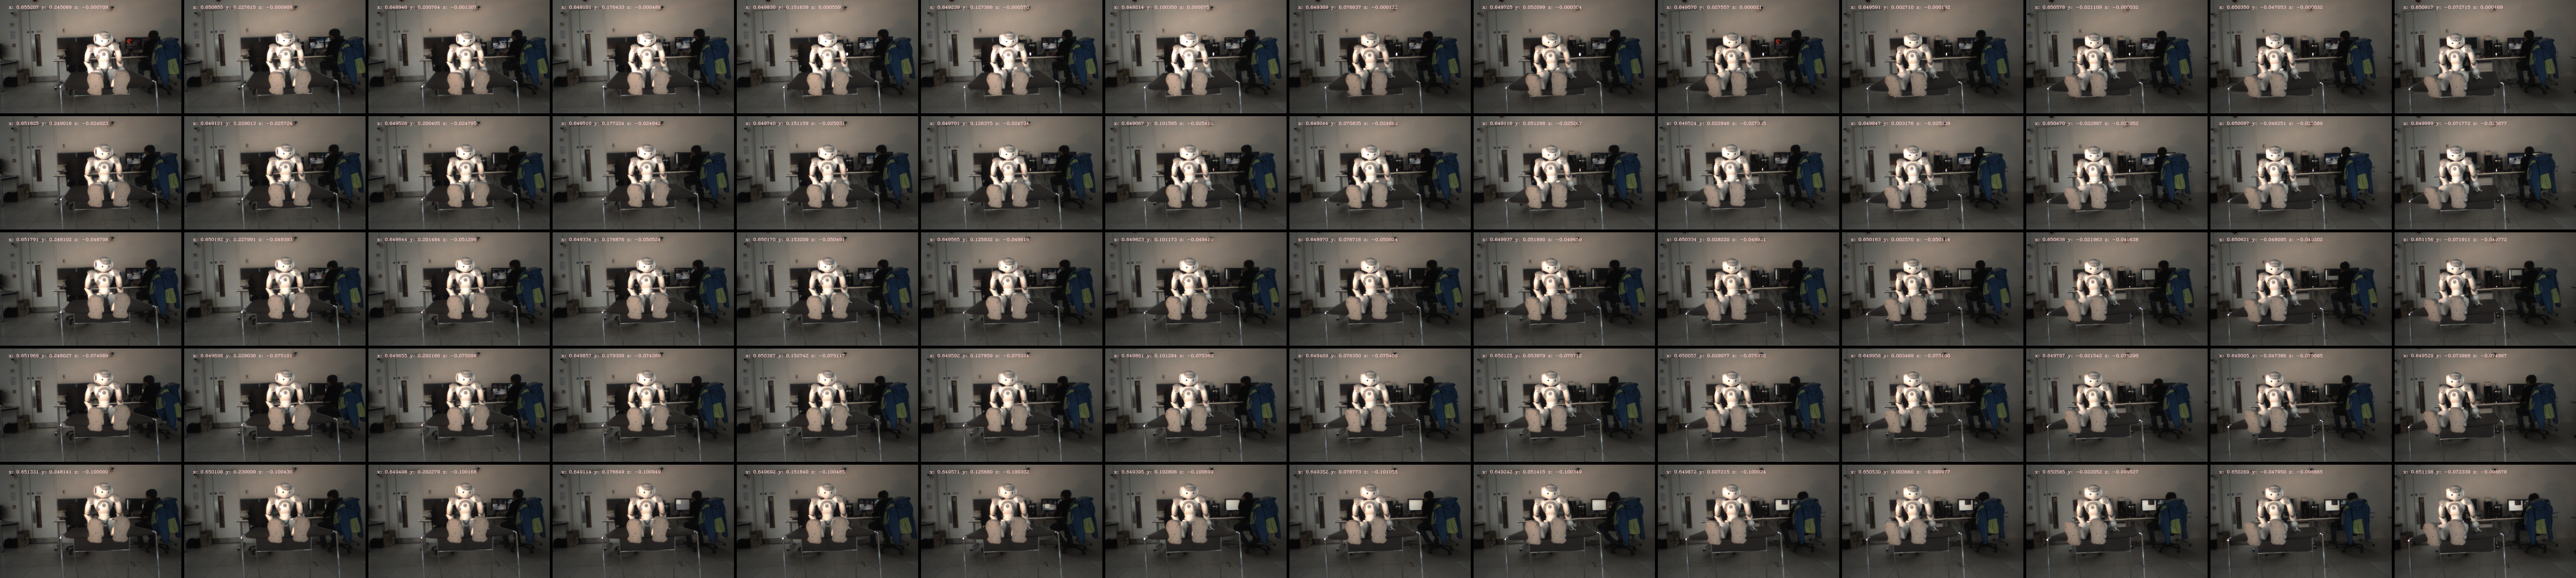
\includegraphics[scale=0.045]{mosaic.jpg}
	\caption{This mosaic is a compilation of all the images taken during one light field acquisition session with the baxter robot.}
	\label{fig:nau_collected_images}
\end{figure}
There were a number of other light fields collected in a similar manner, each of which had varied scene parameters. While the light field in figure \ref{fig:nau_collected_images} is superior to the other collected light fields, it was a beneficial experiment in understanding what a good light field might look like. In other collected light fields, a plastic skull was used in place of the nau. Lighting and distance were also varied, resulting in approximately ten light fields being collected for experimentation. 

\begin{figure}[!ht]
	\centering
	\includegraphics[scale=0.2]{raytrix_raw.png}
	\caption{A depiction of the second renderer based on \cite{Isaksen01} and showing the plane of focus $F$ and the rays coming from it that would be considered in focus.}
	\label{fig:raytrix_raw}
\end{figure}
More recently, a Raytrix r5 camera was acquired and has been used to capture light fields as well. A raw example of this can be seen in figure \ref{fig:raytrix_raw}. In it, the microlenses can clearly be seen, resulting in an almost honeycomb like appearance in the resulting image. The image, being raw, has not gone through any of the software processing similar to that described in the \emph{Light Field Photography} section of the report. Therefore, the image is purely the output from the high resolution image sensor.

\section{System Built}
The following section describes light field renderers that have been successfully constructed to date. Three different systems have been built and iterated upon, and utilize three distinct methods for storing rays and querying a database for the appropriate ray parameters. The first system built takes its form from the seminal paper by Levoy and *** \cite{Levoy96}, the second is based on the work by Isaksen *** \cite{Isaksen01}, and the third is a combination of the work by LEvoy *** and the renderer created by the New Stanford Light Field Archive \cite{lfArchive} **cite Stanford archive.

also assumes that the pixel is a sum of the rays at that point

\begin{figure}[!ht]
	\centering
	\includegraphics[scale=0.7]{mobile_focus.png}
	\caption{A depiction of the second renderer based on \cite{Isaksen01} and showing the plane of focus $F$ and the rays coming from it that would be considered in focus.}
	\label{fig:mobile_focus}
\end{figure}
The first renderer utilizes the common, and original two-plane parameterization set forward in \cite{Levoy96}. As with all parameterizations, a pinhole model is assumed for the camera being used. A number of known values are required for this particular parameterization to work, such as distance of the subject from the camera. With this knowledge, the $ST$ and $UV$ planes may be appropriately placed such that light rays from the subject pass through both before entering the camera. Aside from the distance to the subject, the internal physical camera parameters must be known, such as the size of the image sensor, the camera flange focal length, the position of the camera in a global reference frame, and the number of pixels on the image sensor. Knowing these parameters allows for the storage of two points which are defined by the two planes $P=(S,T), Q=(U,V)$, and together give the direction of the ray along with its recorded intensity value. The new ray database can then be queried at any time for a new camera position. With the new position, a k-Nearest Neighbors (KNN) algorithm is used to compare ray directions with stored directions and an average is taken of intensity values for the nearest rays to create a new image.

\begin{figure}[!ht]
	\centering
	\includegraphics[scale=0.4]{nau_lf.png}
	\caption{A screenshot of the light field interface in action, with the subaperture views shown in blue, the aperture shown as the red circle, and the resulting image shown in the larger window.}
	\label{fig:light_field_system}
\end{figure}

\begin{figure}[!ht]
	\centering
	\begin{minipage}{0.45\textwidth}
		\centering
		\includegraphics[scale=0.30]{nau_occluding.png}
		\caption{The dense camera array used at Stanford to capture a number of light fields.}
		\label{fig:nau_occluding}
	\end{minipage}\hfill
	\begin{minipage}{0.45\textwidth}
		\centering
		\includegraphics[scale=0.30]{seethrough_nau.png}
		\caption{Another collection method, the gantry effectively mimics the camera array so long}
		\label{fig:seethrough_nau}
	\end{minipage}
\end{figure}
The second renderer built is based on \cite{Isaksen01}. It is similar to the previous method but moves the planes to the internals of the camera where there are still no occlusions. Regardless of the plane locations, rays from the scene are still calculated and stored the same way, but there is the addition of a mobile "focus plane". This focus plane allows for focus at different points in the scene via finding the rays coming from the object at the plane position as illustrated in figure \ref{fig:mobile_focus}.

A third renderer was built based on the online viewer found on the New Stanford Light Field Archive website \cite{lfArchive}. After downloading the ActionScript/MXMLsource code and reverse engineering tt, it was rewritten in C++ and OpenCV. It is pictured in figure \ref{fig:light_field_system}. It is a much simplified version of the first renderer that was programmed, but is considerably faster in its run time. In this case, the images are required to be taken specifically from a single plane as any deviation would lead to ghosting. This is caused by the fact that the current rendering technique that this is based on 

\chapter{Proposed Research}

The research done to date has a very natural next step which will be the primary focus of this research, and that is dynamic light fields. The function on which the light field is based on, the plenoptic function, contains seven parameters, one of which is time. Bringing time further into the research of light fields gives the area considerably farther reaching potential in terms of applications. For example, a light field could be used for sports games, where a spectator might want a particular view. This of course, is the easy sell. Deeper applications might include medical imaging, where a patient is situated in an environment where a light field might be collected over time, allowing the attending physician to view and change viewpoints over a patient. Doing this in time would allow the observer to check for changes to the patients health more easily. In research, botanists might want to capture the dynamic light field of a plant from seed to adult, and take different viewpoints through time. Clearly, there are many applications, few to none of which have been adequately explored in the reviewed literature. As well, it is a goal to assemble a modern archive of light fields, both dynamic and static for use by other researchers. These efforts have already begun, as shown in the \emph{Collected Light Fields} section of the \emph{Progress to Date} chapter.

This subject is only lightly covered in the literature review section due to the fact that there is limited research on the topic. For what results there are, the sources that actually cover something akin to dynamic light fields, the apparatus are similarly impractical to those of the early light field capture systems, such as that seen in figure \ref{fig:lytro_immerge}. As well, Lytro's system is only capable of looking out at a scene, which is impractical to impossible for the potential applications mentioned in the previous paragraph. 

\section{First Step: Automated Unstructured Light Fields}
The first step is based on the paper by Davis et al \cite{Davis12}. In the paper, the authors create a light field collection system that is "unstructured", or one in which the camera positions are not fixed in a grid. This is accomplished by using PTAM alongside a graphical user interface to instruct a human on where to move the hand held camera. The authors are able to use PTAM as the renderer they use does not require the precise position measurements, similar to that of the third renderer discussed in the \emph{Systems Built} section. Utilizing the supposed much improved slam technique, ORB-SLAM2, it may be possible to acquire precise enough location data for the camera. It is intended, however, to use the PR2 robot developed by Willow Garage in place of a human, thereby automating and likely streamlining the procedure. An image of the PR2 can be seen in figure \ref{fig:pr2_image}. The precision and accuracy of the PR2 will likely be enough to collect light field data sufficient for the first two renderers discussed in the \emph{Systems Built} section.

\begin{figure}[!ht]
	\centering
	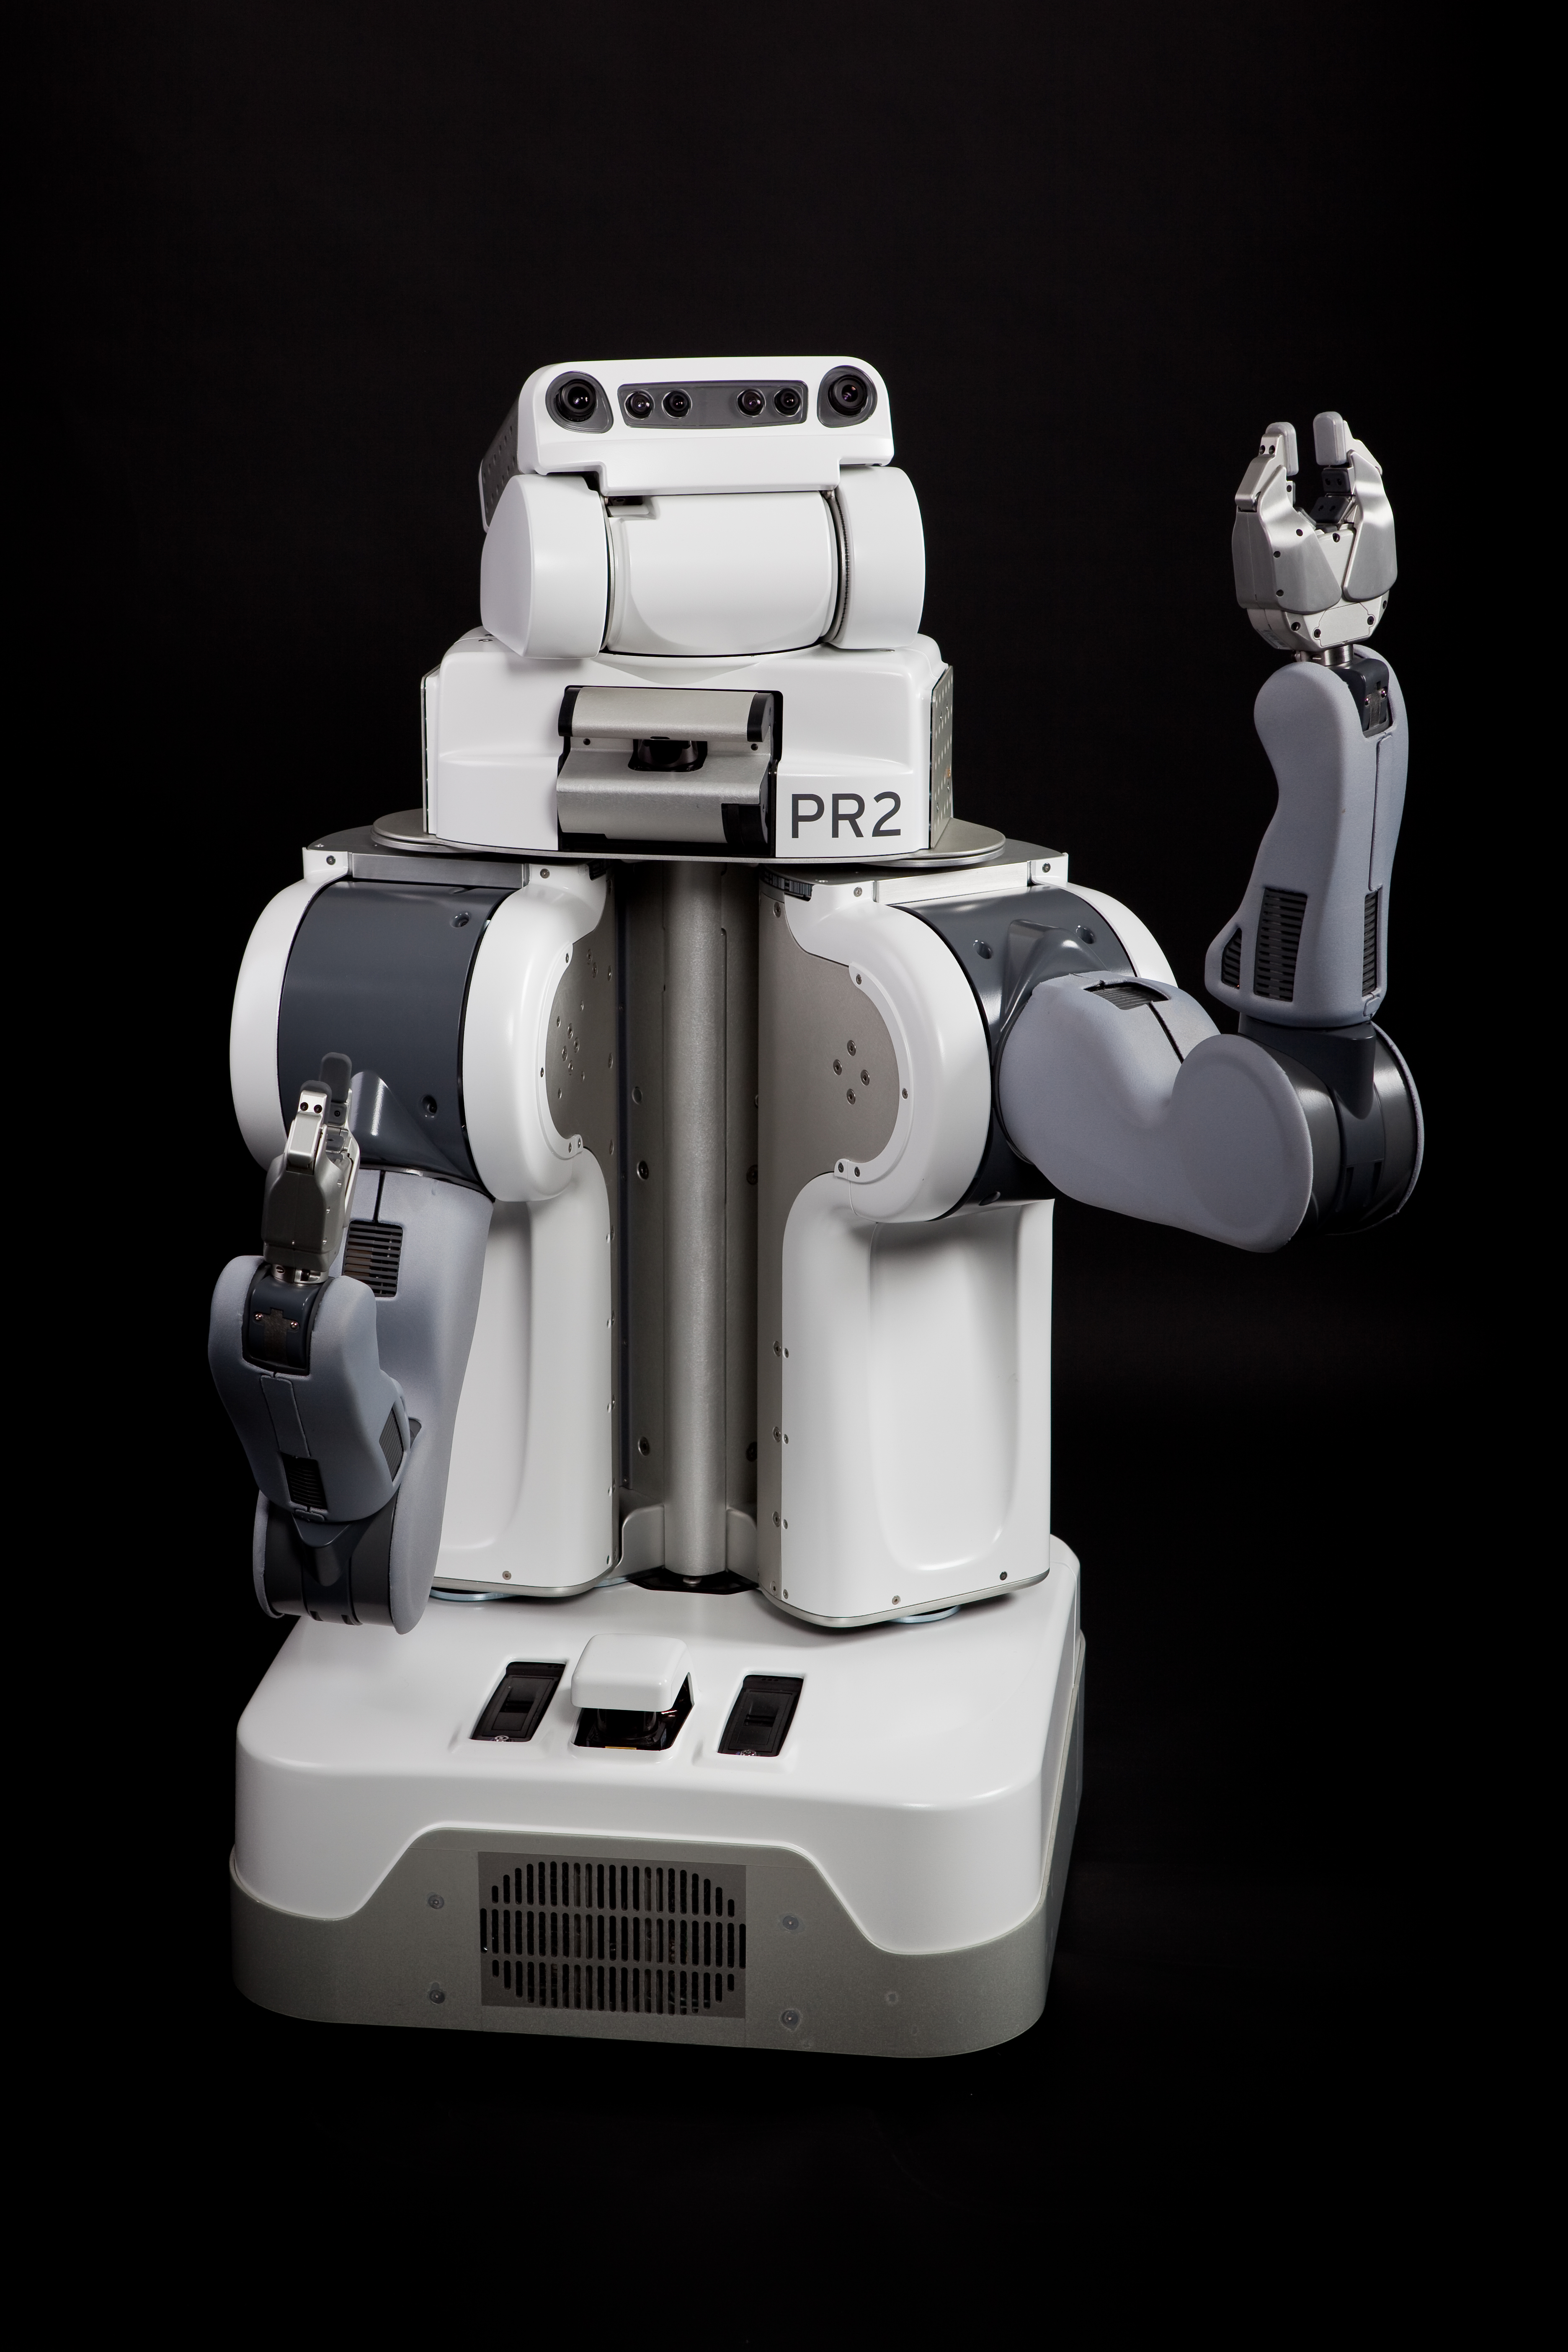
\includegraphics[scale=0.08]{pr2_image.jpg}
	\caption{A screenshot of the light field interface in action, with the subaperture views shown in blue, the aperture shown as the red circle, and the resulting image shown in the larger window.}
	\label{fig:pr2_image}
\end{figure}
While the PR2 might have a superior position estomator, ORB-SLAM2 could still be very useful on board a drone. A drone has its own advantages, such as being able to collect the light field for hard to reach locations that might need to be maintained, such as cooling towers or chimneys. There are existing drones that can easily be controlled from the computer and capture data, such as the ARDrone pictured in figure \ref{fig:ardrone_image}. With the SLAM system in place, it would be a natural, and relatively easy, step further from the PR2 based system. As well, it would possible to incorporate a swarm of drones into the data collection process which would be especially useful for light field acquisition for sporting events.

\begin{figure}[!ht]
	\centering
	\includegraphics[scale=0.4]{ardrone_image.png}
	\caption{A screenshot of the light field interface in action, with the subaperture views shown in blue, the aperture shown as the red circle, and the resulting image shown in the larger window.}
	\label{fig:ardrone_image}
\end{figure}

This step will differ considerably from Davis' paper in the way in which the light field is actually collected. Rather than using a single webcam held by a person relying on a graphical interface to indicate where the user should move the camera, a robot will use one or more cameras and inherently (via the programming) know where to move the cameras to get the appropriate data. The idea behind this is that in moving the collection process to a robot, it can be accomplished much more efficiently. As well, more exact camera locations can be defined which naturally moves into the second step.

\section{Second Step: Completing Light Fields}
With the large amount of data required for a light field, let alone a dynamic light field, the first attempts at a system will be offline. One of the key steps towards accomplishing the overall goal is utilizing the research already done on minimizing data required for creating light fields see ***. Some of these methods have been covered in the literature review section of this report. It is intended that several of the existing methods will be implemented on collected light fields, steadily removing data to better understand which method is best suited for sparsely sampled light fields.

One of the first methods to be attempted will be that presented by Mahajan \emph{et al} in their paper \emph{Moving Gradients: A Path-Based Method for Plausible Image Interpolation}

The next would be in the realm signal processing

The third would be a deep learning method. 

With the methodology in placing for collecting light fields from the first step, the second, and more complicated step can commence. In it, methods from papers such as Light***Fields and Convolutional Neural Networks etc are employed to fill in the data from the previous step.

\section{Next Steps}

With the knowledge and infrastructure in place from the previous steps, a number of avenues open up for applications of the technology. These can range anywhere from the medical field to construction where an accurate and immersive virtual scene of the area of interest is available.

It is hoped that these light fields can be archived and used interchangeably in tim

\chapter{Conclusion}

The ability to allow a user to move through space and time could have huge implications in the realm of science and industry, allowing scietists to monitor experiments more closely than ever, and industry to monitor apparatus more in depth and with greater detail than before.

In the event this is required...
This report has introduced the concept of the light field as well gone through a comprehensive review of the literature on the subject. A proposal has been set forth in which research will be done to further explore the potential of light field video and its potential uses. 

A considerable amount of work has been done to date, from programming and operating the humanoid Baxter robot and experimenting with SLAM, to capturing multiple light fields and utilizing different methods to visualize them. This work done has effectively laid the foundation for the phases to come that have been laid out in the NEx Steps section of the report.

Utilizing the papers *** will be key in collecting sufficient data to support light field video *** do we want to call it something else? Also, probably should lay this out more like the structure of the paper...


\begin{thebibliography}{10}%Any two digit number for more than nine references

\bibitem{Adelson91}
	Adelson, Edward H. \emph{The Plenoptic Function and Elements of Early Vision} (1991). Computational Models of Visual Processing, pp. 3-20.

\bibitem{Anderson16}
	Anderson, R., Gallup, D., Barron, J. T., Kontkanen, J., Snavely,  N., Hernandez, C., Agarwal, S., and Seitz, S. M., \emph{Jump: Virtual Reality Video} (2016). SA '16 Technical Papers.

\bibitem{Bolles87}
	Bolles, R. C., Baker, H. H., and Marimont, D. H., \emph{Epipolar-Plane Image Analysis: An Approach to Determining Structure from Motion} (1987). International Journal of Computer Vision, no. 1, pp. 7-55. 

\bibitem{Camahort09}
	Camahort, E., Abad, F. and Fussell, D., \emph{A line-space analysis of light-field representations} (2009). Graphical Models. no. 71. pp. 168-183.

\bibitem{Chai00}
	Chai, J., Tong, X., Chan, S., and Shum, H., \emph{Plenoptic Sampling} (2000). SIGGRAPH '00, pp. 307-318.

\bibitem{Davis12}
	Davis, A., Levoy, M., and Durand, F., \emph{Unstructured Light Fields} (2012). Eurographics 2012, no. 31.

\bibitem{Engel12}
	Engel, J., Sturm, J., and Cremers, D., \emph{Accurate Figure Flying with a Quadrocopter Using Onboard Visual and Inertial Sensing} (2012). IEEE/RJS International Conference on Intelligent Robot Systems, no. 320.

\bibitem{Georgeiv06}
	Georgeiv, T., Zheng, K. C., Curless, B., Salesin, D., Nayar, S., and Intwala, C., \emph{Spatio-Angular Resolution Tradeoff in Integral Photography} (2006). Eurographics Symposium on Rendering

\bibitem{Gortler96}
	Gortler, S. J., Grzeszczuk, R., Szeliski, R., and Cohen, M. F., \emph{The Lumigraph} (1996). SIGGRAPH '96, pp. 43-54.
	
\bibitem{Huang14}
	Huang, Z. and Sanderson, A., \emph{Light field modelling and interpolation using Kriging techniques}	(2014). Society of Light and Lighting, no. 46, pp. 219-237.
	
\bibitem{Ihrke16}
	Ihrke, I., Restrepo, J. and Mignard-Debise, L., \emph{Principles of Light Field Imaging} (2016). IEEE Signal Processing Magazine.
	
\bibitem{Isaksen01}
	Isaksen, A., McMillan, L., and Gortler, S. J., \emph{Dynamically Reparameterized Light Fields} (2000). SIGGRAPH '00, pp. 297-306.

\bibitem{Jachnik13}
	Jachnik, J., Newcombe, R. A., Davison, A. J., \emph{Real-Time Surface Light-field Capture for Augmentation of Planar Specular Surfaces} (2013). ISMAR.
	
\bibitem{Joubert15}
	Joubert, N., Roberts, M., Truong, A., Berthouzoz, F. and Hanrahan, P., \emph{An Interactive Tool for Designing Quadrotor Camera Shots} ACM Transactions on Graphics, no. 34. 

\bibitem{Kalantari16}
	Kalantari, N. K., Wang, T. and Ramamoorthi, R., \emph{Learning-Based View Synthesis for Light Field Cameras} (2016). SIGGRAPH Asia '16.

\bibitem{Katayama95}
	Katayama, A., Tanaka, K., Oshino, T. and Tamura, H., \emph{A Viewpoint Dependent Stereoscopic Display Using Interpolation of Multi-Viewpoint Images} (1995). SPIE. no. 2409.
	
\bibitem{Kim13}
	Kim, C., Zimmer, H., Pritch, Y., Sorkine-Hornung, A. and Gross, M., \emph{Scene Reconstruction from High Spatio-Angular Resolution Light Fields} (2013). ACM Trans. Graph.	
	
\bibitem{Klein07}
	Klein, G. and Murray, D., \emph{Parallel Tracking and Mapping for Small AR Workspaces} (2007). ISMAR 2007. 	

\bibitem{Koller04}
	Koller, D., Turitzin, M., Levoy, M., Croccia, G., Cignoni, P. and Scopigno, R., \emph{Protected Interactive 3D Graphics via Remote Rendering} (2004). no. 23. pp. 695-703.

\bibitem{Levoy96}
	Levoy, M. and Hanrahan, P., \emph{Light Field Rendering} (1996). SIGGRAPH '96.
	
\bibitem{Levoy06a}
	Levoy, M., \emph{Light Fields and Computational Imaging} (2006). Computer. no. 39. pp. 46-55.

\bibitem{Levoy06b}
	Levoy, M., Ng, R., Adams, A., Footer, M. and Horowitz, M., \emph{Light Field Microscopy} (2006). SIGGRAPH '06. pp. 924-934.
	
\bibitem{Mahajan09}
	Mahajan, D., Huang, F., Matusik, W. and Bulhumeur, P. N., \emph{Moving Gradients: A Path-Based Method for Plausible Image Interpolation} (2009). ACM Transactions on Graphics 28.	
	
\bibitem{McMillan95}
	McMillan, L. and Bishop, G., \emph{Plenoptic Modelling: An Image-Based Rendering System} (1995). SIGGRAPH '95. pp. 39-46.

\bibitem{Mur-Artal15}
	Mur-Artal, R., Montiel, M. M. and Tardos, J. D., \emph{ORB-SLAM: a Versatile and Accurate Monocular SLAM System} (2015). IEEE Transactions on Robotics. no. 31.

\bibitem{Ng05}
	Ng, R., Levoy, M., Bredif, M., Duval, G., Horowitz, M. and Hanrahan, P. \emph{Light Field Photography with a Hand-held Plenoptic Camera} (2005). Stanford Tech Report CTSR. no. 2.

\bibitem{Ng06}
	Ng, Ren, \emph{Digital Light Field Photography.} (2006). PhD thesis, Stanford University.	

\bibitem{Oberlin16}
	Oberlin, J. and Tellex, S., \emph{Time-Lapse Light Field Photography With a 7 DoF Arm} (2016). RSS Workshop on Geometry and Beyond - Representations, Physics, and Scene Understanding for Robots. 

\bibitem{Perwass12}
	Perwass, C. and Wietzke, L., \emph{Single Lens 3D-Camera with Extended Depth-of-Field} (2012). Proceeding of SPIE.

\bibitem{Roberts16}
	Roberts, M. and Hanrahan, P., \emph{Generating Dynamically Feasible Drone Trajectories for Quadrotor Cameras} (2016). SIGGRAPH '16.

\bibitem{Shi14}
	Shi, L., Hassanieh, H., Davis, A., Katabi, D. and Durand, F., \emph{Light Field Reconstruction Using Sparsity in the Continuous Fourier Domain} (2014). ACM Transactions on Graphics. no. 34.

\bibitem{Shum01}
	Shum, H. and Kang, S., \emph{A Review of Image-based Rendering Techniques} (2001). Institute of Electrical and Electronic Engineers, Inc.

\bibitem{Srikanth14}
	Srikanth, M., Bala, K. and Durand, F., \emph{Computational Rim Illumination with Aerial Robots} (2014). Proceeding of the Workshop on Computational Aesthetics. pp. 57-66.

\bibitem{Vaish06}
	Vaish, V., Levoy, M., Szeliski, R., Zitnick, C. L. and Sing, B., \emph{Reconstructing Occluded Surfaces using Synthetic Apertures: Stero, Focus, and Robust Measures} (2006). no. 2. pp. 2331-2338.
	
\bibitem{Wilburn05}
	Wilburn, B., Joshi, N., Vaish, V., Levoy, M. and Horowitz, M., \emph{High-Speed Videography Using a Dense Camera Array} (2004). Computer Vision and Pattern Recognition.

\bibitem{lfArchive}
	Stanford New Light Field Archive http://lightfield.stanford.edu/

\bibitem{ardrone}
	ARDrone https://www.parrot.com/fr/drones/

\bibitem{baxter}
	Baxter Robot http://www.rethinkrobotics.com/baxter/
	
\bibitem{lytro}
	Lytro Immerge https://www.lytro.com/immerge
	
\bibitem{PR2}
	PR2 Robot http://www.willowgarage.com/pages/pr2/overview
	
\bibitem{Raytrix}
	Raytrix Camera https://www.raytrix.de/
	
\bibitem{Personal}
	Personal Source

\end{thebibliography}

\end{document}